\documentclass{article}

\usepackage{microtype}
\usepackage{booktabs}
\usepackage{balance}
\usepackage{graphicx}
\usepackage{xcolor}
\usepackage{tikz}
\usetikzlibrary{arrows.meta,backgrounds,fit,positioning}
\usepackage{hyperref}
\newcommand{\theHalgorithm}{\arabic{algorithm}}
\usepackage[accepted]{../report/icml2025}
\setcitestyle{numbers,square}

\definecolor{TUred}{RGB}{165,30,55}
\definecolor{TUdark}{RGB}{50,65,75}
\definecolor{TUblue}{RGB}{0,105,170}
\definecolor{TUgold}{RGB}{180,145,45}
\definecolor{TUgreen}{RGB}{80,135,80}
\newcommand{\reporttodo}[1]{{\small\textcolor{TUred}{\textbf{TODO:} #1}}}

\hypersetup{
  colorlinks=true,
  hypertexnames=false,
  linkcolor=TUblue,
  citecolor=TUblue,
  urlcolor=TUblue
}

\setlength{\floatsep}{6pt}
\setlength{\textfloatsep}{7pt}
\setlength{\intextsep}{5pt}
\setlength{\abovecaptionskip}{3pt}
\setlength{\belowcaptionskip}{0pt}

\icmltitlerunning{Focused Hybrid Retrieval for Tübingen}

\begin{document}

\twocolumn[
\icmltitle{Focused Hybrid Retrieval for English Tübingen Web Content}

\begin{icmlauthorlist}
\icmlauthor{INFO4271 project group}{equal}
\end{icmlauthorlist}

\icmlaffiliation{equal}{University of Tübingen}
\icmlkeywords{focused crawling, information retrieval, hybrid search, search interface}
\vskip 0.15in
]

\begin{abstract}
We present an end-to-end search engine for English web content related to
Tübingen. The system combines a resumable focused crawler, a self-implemented
BM25F first stage, semantic second-stage re-ranking, batch retrieval, and an
interactive result interface. In a diagnostic 20-query ablation, semantic
re-ranking improves nDCG@10 from .7038 to .7342, while the evaluated proximity
bonus does not improve effectiveness. The final retrieval configuration
therefore uses BM25F followed by semantic re-ranking.
\end{abstract}

\section{Introduction}
The project requires a local search engine for English Tübingen-related web
content. It must cover crawling, indexing, retrieval of 100 results, batch
evaluation, and an interface that goes beyond a conventional ranked list. Our
system implements this complete pipeline and uses semantic re-ranking as its
retrieval innovation. This report describes the main design choices and uses a
controlled ablation to justify the final ranking configuration.

\section{System Overview}
The system separates offline collection and indexing from online retrieval.
The crawler stores accepted pages locally, after which the indexer constructs a
field-aware lexical index and document embeddings. At query time, BM25F
retrieves 100 candidates. A semantic model scores only these candidates, and
the fused ranking is returned through the API, batch command, and interactive
interface.

\reporttodo{Add the immutable repository link before submission.}

\section{Focused Crawling and Storage}
\subsection{Crawl Strategy}
Seeds were selected manually, favoring aggregator pages expected to expose
many relevant outgoing links. The focused crawler prioritizes links that are
likely to lead to Tübingen-related content. It respects
\texttt{robots.txt} and restricts the collection to English pages. Multiple
workers consume a global priority frontier organized into per-host queues,
with at most one active request per host. Host cooldowns, page caps, and early
stopping after repeated rejects prevent individual domains from dominating the
collection.
Separately, Serper, a Google Search results API, was used to discover pages
for offline \textsc{PageVerdict} labeling; it is not part of the runtime crawl
loop \citep{serper}.

\subsection{Learned Focus Control}
\textsc{LinkVerdict} prioritizes discovered links before fetching, whereas
\textsc{PageVerdict} decides whether a fetched page enters the collection.
Initial experiments used fixed heuristics. Qualitative inspection suggested
that these rules were too rigid for the varied links and content relevant to
Tübingen, motivating learned models for both decisions.
Figure~\ref{fig:verdict-training} summarizes their offline training, and
Figure~\ref{fig:crawler-runtime} shows their roles in the crawl loop.
Table~\ref{tab:verdict-benchmark} reports their human-label test performance.
For \textsc{PageVerdict}, Qwen~2.5:7B labels provide weak supervision alongside
human labels; \textsc{LinkVerdict} uses human labels only because qualitative
experiments with the more limited link context were less reliable. The
manually labeled, host-disjoint PageVerdict comparison set contains 147 hosts
and deliberately emphasizes model disagreements. In Table~\ref{tab:verdict-benchmark},
Q+H denotes Qwen plus human training labels and H denotes human labels only.

\begin{figure}[t]
  \centering
  \resizebox{\columnwidth}{!}{%
  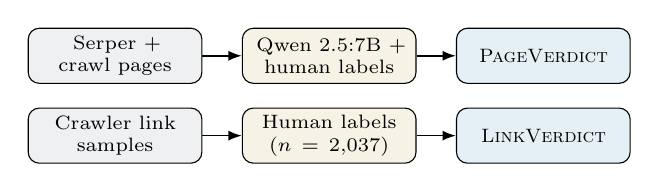
\begin{tikzpicture}[
    baseline=(current bounding box.south),
    node distance=3mm and 5mm,
    box/.style={
      draw,
      rounded corners,
      align=center,
      font=\scriptsize,
      minimum height=7mm,
      text width=21mm,
      inner sep=1.5pt
    },
    arrow/.style={-{Latex[length=1.7mm]}, semithick}
  ]
    \node[box, fill=TUdark!8] (page-samples) {Serper +\\crawl pages};
    \node[box, fill=TUgold!12, right=of page-samples] (page-labels)
      {Qwen 2.5:7B +\\human labels};
    \node[box, fill=TUblue!10, right=of page-labels] (page-model)
      {\textsc{PageVerdict}};

    \node[box, fill=TUdark!8, below=of page-samples] (link-samples)
      {Crawler link\\samples};
    \node[box, fill=TUgold!12, right=of link-samples] (link-labels)
      {Human labels\\($n=2{,}037$)};
    \node[box, fill=TUblue!10, right=of link-labels] (link-model)
      {\textsc{LinkVerdict}};

    \draw[arrow] (page-samples) -- (page-labels);
    \draw[arrow] (page-labels) -- (page-model);
    \draw[arrow] (link-samples) -- (link-labels);
    \draw[arrow] (link-labels) -- (link-model);
  \end{tikzpicture}
  }
  \caption{Offline training of the TF--IDF logistic-regression verdict models.}
  \label{fig:verdict-training}
\end{figure}

\begin{figure}[t]
  \centering
  \resizebox{\columnwidth}{!}{%
  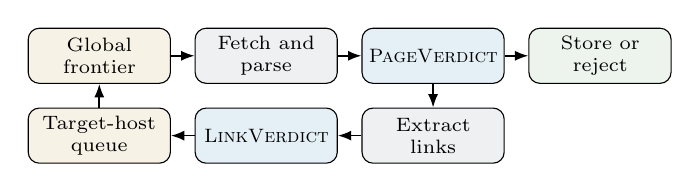
\begin{tikzpicture}[
    baseline=(current bounding box.south),
    node distance=3mm,
    box/.style={
      draw,
      rounded corners,
      align=center,
      font=\scriptsize,
      minimum height=7mm,
      text width=17mm,
      inner sep=1.5pt
    },
    arrow/.style={-{Latex[length=1.7mm]}, semithick}
  ]
    \node[box, fill=TUgold!12] (frontier) {Global\\frontier};
    \node[box, fill=TUdark!8, right=of frontier] (fetch) {Fetch and\\parse};
    \node[box, fill=TUblue!10, right=of fetch] (page)
      {\textsc{PageVerdict}};
    \node[box, fill=TUgreen!10, right=of page] (decision)
      {Store or\\reject};

    \node[box, fill=TUgold!12, below=of frontier] (queue)
      {Target-host\\queue};
    \node[box, fill=TUblue!10, below=of fetch] (link)
      {\textsc{LinkVerdict}};
    \node[box, fill=TUdark!8, below=of page] (extract)
      {Extract\\links};

    \draw[arrow] (frontier) -- (fetch);
    \draw[arrow] (fetch) -- (page);
    \draw[arrow] (page) -- (decision);
    \draw[arrow] (page) -- (extract);
    \draw[arrow] (extract) -- (link);
    \draw[arrow] (link) -- (queue);
    \draw[arrow] (queue) -- (frontier);
  \end{tikzpicture}
  }
  \caption{Runtime crawl loop. \textsc{LinkVerdict} scores extracted links
  before admission to the target host queue.}
  \label{fig:crawler-runtime}
\end{figure}

\subsection{Persistence and Collection Statistics}
URLs are normalized and deduplicated before entering the frontier. After
fetching, a 64-bit SimHash over token trigrams rejects fingerprints within a
Hamming distance of three from an accepted page \citep{manku2007}.
Accepted HTML is stored locally, while crawl metadata and model decisions are
persisted in SQLite. The frontier and deduplication state can be restored after
interruption.

\begin{table}[t]
  \centering
  \caption{Collection statistics. ``Hosts'' denotes domains with accepted
  pages; duplicates are included among rejected pages.}
  \label{tab:crawl-statistics}
  \small
  \setlength{\tabcolsep}{3.5pt}
  \begin{tabular}{@{}rrrrr@{}}
    \toprule
    Fetched & Accepted & Rejected & Duplicates & Hosts \\
    \midrule
    23,943 & 10,027 & 13,916 & 2,425 & 325 \\
    \bottomrule
  \end{tabular}
\end{table}

The crawler accepted 41.9\% of fetched pages, showing that its focus controls
filtered a substantial share of the explored content.

\begin{table}[t]
  \centering
  \caption{Performance on manually labeled, host-disjoint test sets.}
  \label{tab:verdict-benchmark}
  \small
  \setlength{\tabcolsep}{3pt}
  \begin{tabular}{@{}lrrrrr@{}}
    \toprule
    Model & $n$ & Bal.\ Acc. & F1 & ROC--AUC & AP \\
    \midrule
    Page (Q+H) & 147 & .692 & .709 & .774 & .720 \\
    Page (H) & 147 & .624 & .599 & .719 & .730 \\
    Link (H) & 546 & .746 & .629 & .822 & .627 \\
    \bottomrule
  \end{tabular}
\end{table}

\section{Indexing and Ranking}

\subsection{Lexical Retrieval}
Text is lowercased and split into alphanumeric tokens, excluding single-character
tokens and English stopwords. The inverted index covers body,
title, and URL fields and stores body positions for snippets and proximity
scoring. For term $t$, document $d$, and fields $f$, BM25F computes
\[
\tilde f_{t,d}=\sum_f w_f
\frac{f_{t,d,f}}{1-b+b\,|d_f|/\overline{|d_f|}},
\]
\[
s_{\mathrm{BM25F}}(d,q)=
\sum_{t\in q}\mathrm{IDF}(t)\frac{\tilde f_{t,d}}{k_1+\tilde f_{t,d}}.
\]
We use $b=0.75$ and $k_1=1.2$, preserving term-frequency saturation after
field weighting \citep{robertson2004bm25f}. Based on qualitative experiments,
the body, title, and URL weights are 1, 5, and 3, respectively.

For documents matching at least two distinct query terms, we evaluate a
proximity bonus of $0.25/(1+g)$, where $g$ is the extra gap in the shortest
matching body window. This deliberately weak signal is related to prior
proximity extensions of Okapi scoring \citep{rasolofo2003}. Because the ablation
in Table~\ref{tab:retrieval-ablation} shows no effectiveness gain, the bonus is
not used in the selected configuration.

\subsection{Semantic Retrieval and Fusion}
The second stage uses the general-purpose
\texttt{nli-mpnet-base-v2} encoder, whose sentence-embedding training uses
SNLI and MultiNLI natural-language-inference data
\citep{nli-mpnet-base-v2}. Each document is split into at most 20 overlapping
2,000-character passages, and its title is embedded separately. With cosine
similarity between the query $q$, title $t_d$, and passages $p_i$, the
heuristically weighted semantic score is
\[
\begin{array}{rl}
s_{\mathrm{sem}}(d,q)={}&0.20\cos(q,t_d)\\
&+0.65\max_i\cos(q,p_i)\\
&+0.15\,\mathrm{mean}_{i\in\mathrm{top3}}\cos(q,p_i).
\end{array}
\]
Semantic evidence is computed only for the 100 BM25F candidates. The final
score is
\[
s_{\mathrm{final}}(d,q)=0.7\,\hat{s}_{\mathrm{BM25F}}(d,q)
  +0.3\,s_{\mathrm{sem}}(d,q),
\]
where $\hat{s}_{\mathrm{BM25F}}$ is min--max normalized. We tested mixture
weights in increments of 0.1 and selected 0.7/0.3 because they achieved the
highest nDCG@10.

\section{Evaluation}
To select the final retrieval configuration, we compare BM25F with proximity
scoring and semantic re-ranking in a controlled ablation. All variants use the
same frozen index and 20-query set. The queries were selected manually to cover
broad topics, named entities, and specific tasks across tourism, university
life, mobility, recreation, and local services. We pool the top 20 results from
all four variants, producing 466 unique query--URL pairs, and grade them from 0
(irrelevant) to 3 (highly relevant). The primary metric is nDCG@10; nDCG@20,
MRR@10, and warmed API latency provide complementary evidence.

\begin{table*}[t]
\centering
\caption{Retrieval ablation on 20 queries. All variants use BM25F top-100
candidates; semantic scoring only re-ranks those candidates. The pooled top 20
contains 466 single-assessor judgments with complete judged coverage.
Latency is the mean warmed API response time.}
\label{tab:retrieval-ablation}
\small
\setlength{\tabcolsep}{9pt}
\begin{tabular}{@{}lccrrrr@{}}
\toprule
Variant & Proximity & Semantic & nDCG@10 & nDCG@20 & MRR@10 & ms/query \\
\midrule
BM25F                & no  & no  & .7038 & .8103 & .9500 &  1.90 \\
BM25F + proximity    & yes & no  & .6958 & .8002 & .9500 & 18.13 \\
BM25F + semantic     & no  & yes & \textbf{.7342} & \textbf{.8441} &
  \textbf{.9750} & 64.64 \\
Full                 & yes & yes & .7183 & .8395 & \textbf{.9750} & 64.77 \\
\bottomrule
\end{tabular}
\end{table*}

Semantic re-ranking improves nDCG@10 by .0304 over BM25F, whereas proximity
reduces effectiveness both alone and in the full system. We therefore select
BM25F with semantic re-ranking as the final configuration.

\section{Result Presentation}
The presentation aims to expose retrieved URLs in a more creative form than a
conventional result list. Inspired by the Internet as a network of
interconnected networks, the interface maps results to stellar constellations
through which the user can navigate as a galaxy. The web client presents ten
clickable result cards alongside ten result stars. Star size and color encode
the result-set min--max-normalized final score, while vertical position follows
rank by default. Users may define semantic \(x\)- and \(y\)-axes through
category labels, onto which the server projects centered and bounded document
embeddings. Overlapping stars fan out on hover, and pagination pans the camera
between result constellations. The spatial view augments the ranked cards
without altering retrieval order.

\begin{figure*}[t]
  \centering
  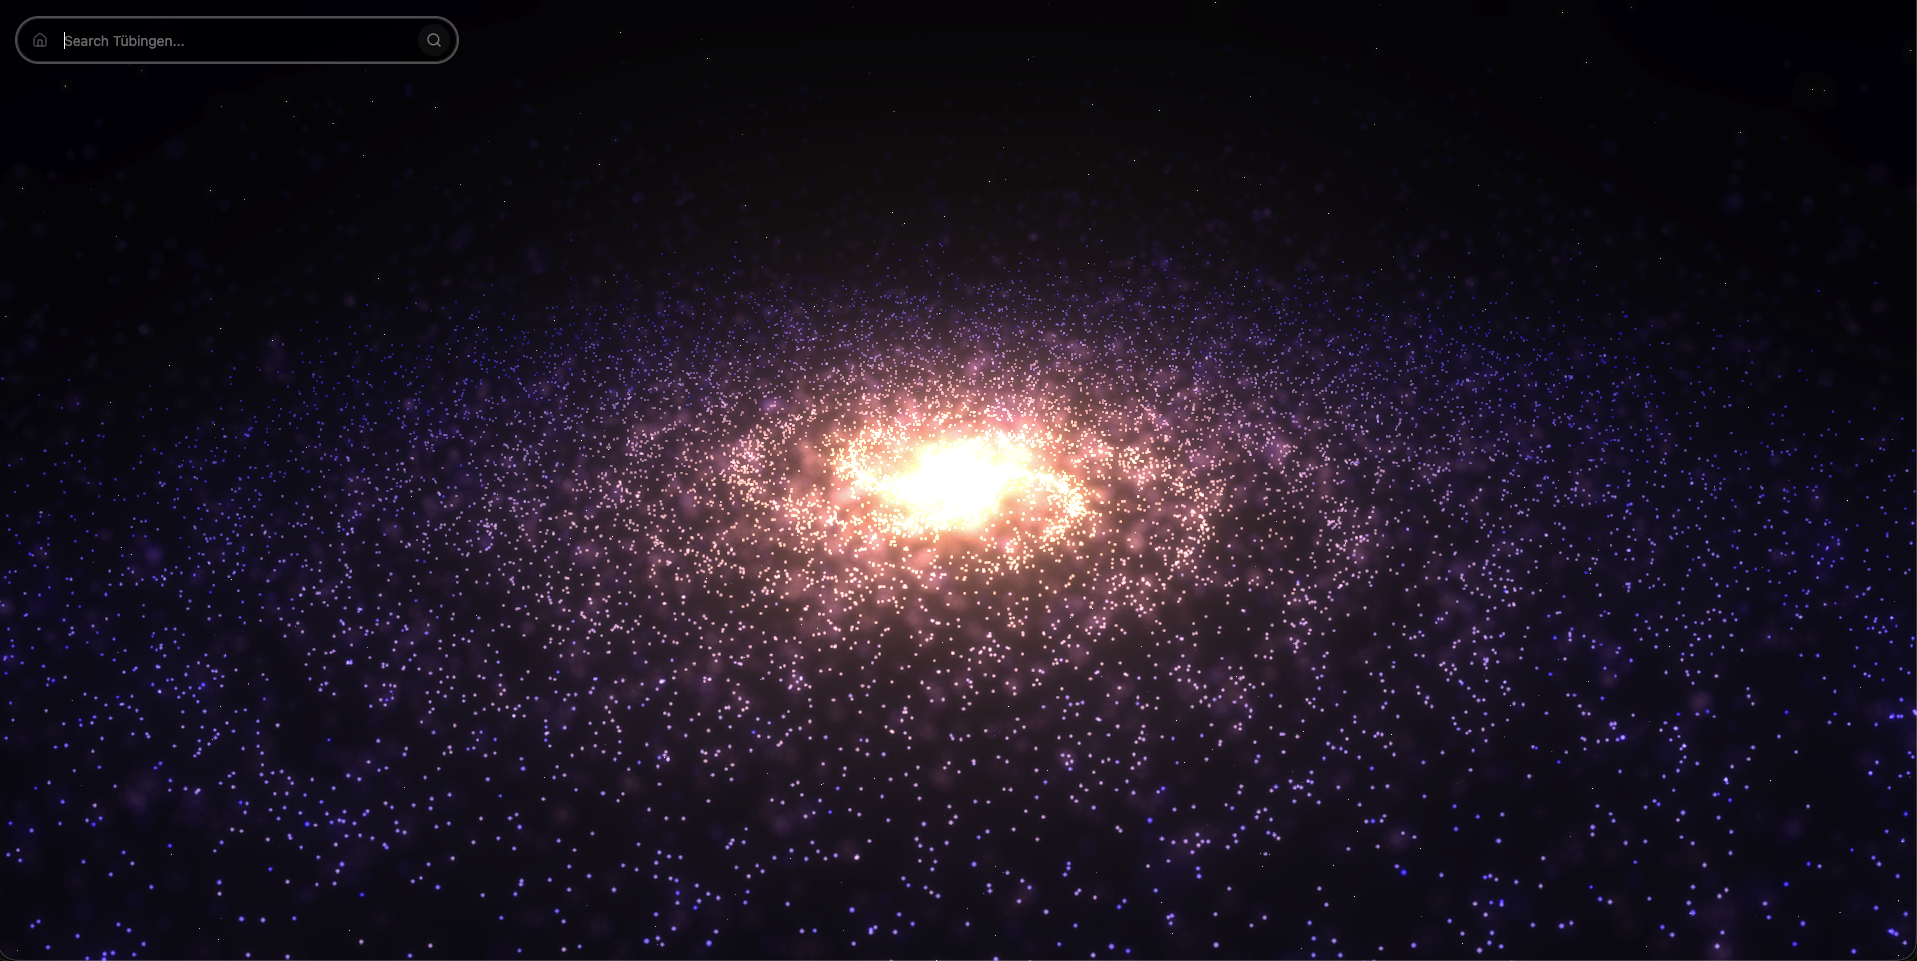
\includegraphics[width=\textwidth]{img/start_screen.png}\\[-1mm]
  {\scriptsize (a) Query entry.}\\[2mm]
  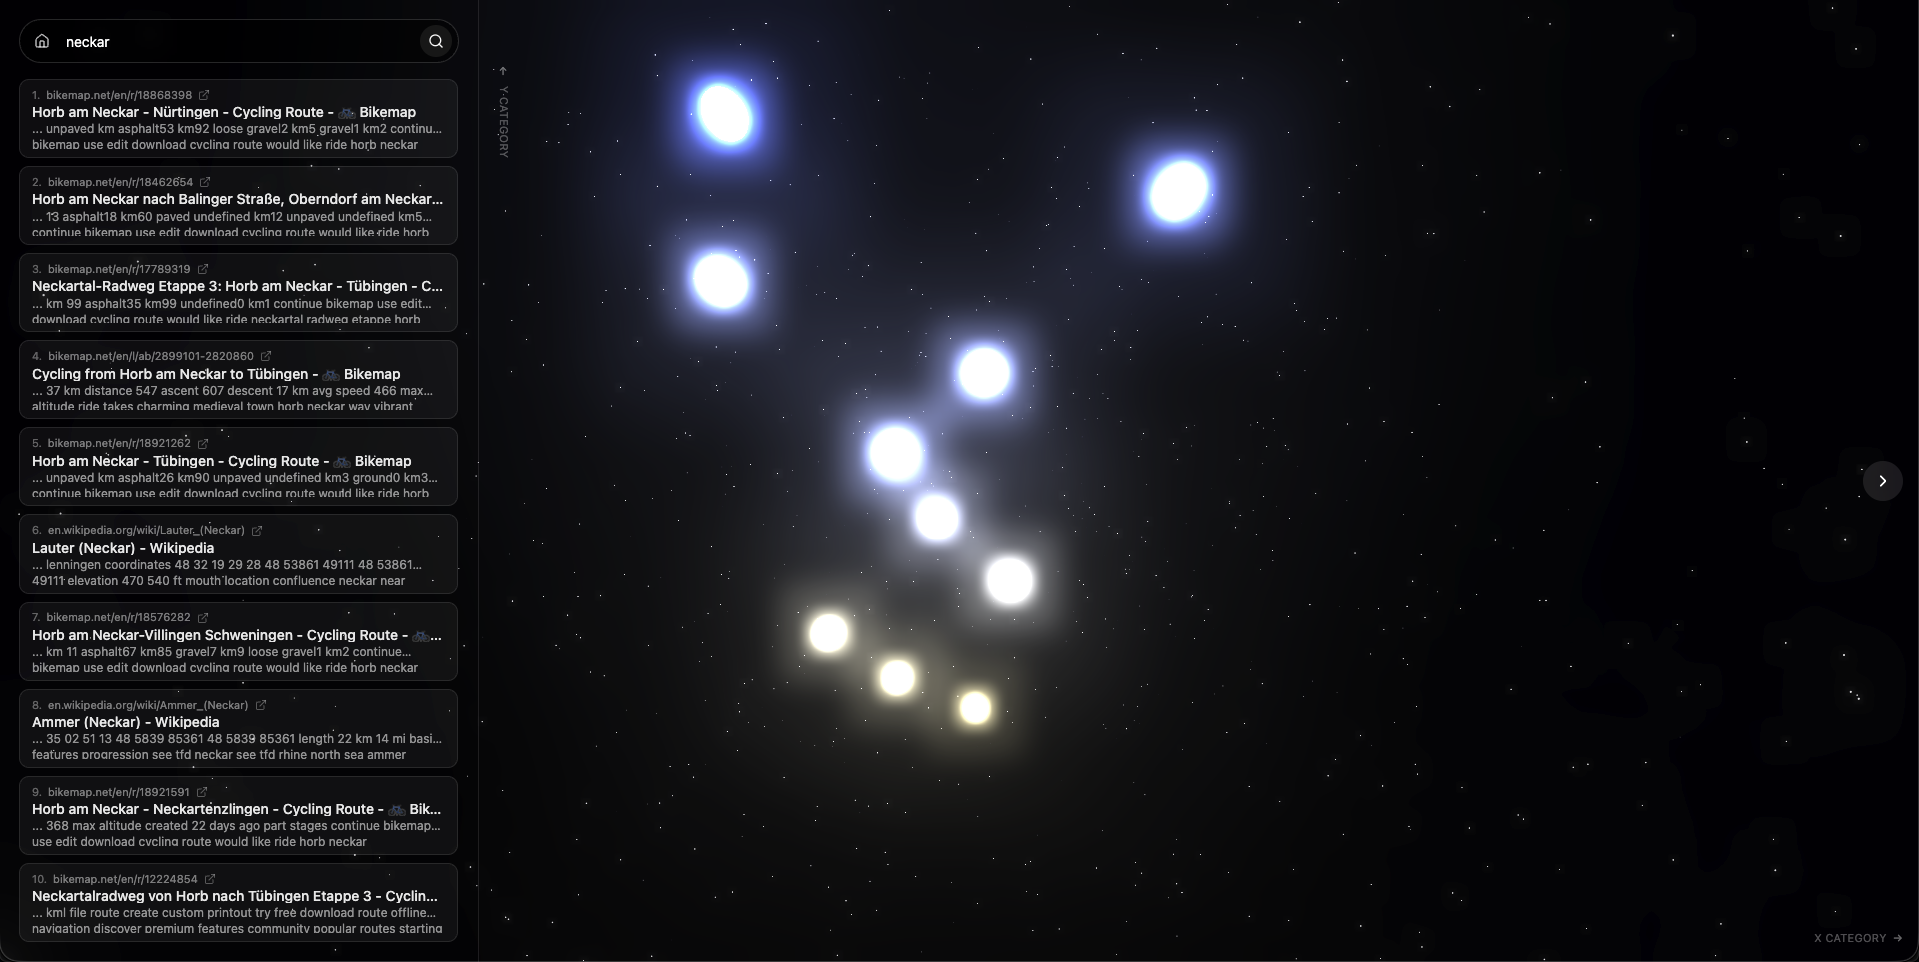
\includegraphics[width=\textwidth]{img/result_screen.png}\\[-1mm]
  {\scriptsize (b) Ranked cards and interactive result constellation.}
  \caption{Implemented search interface.}
  \label{fig:interface}
\end{figure*}

\section{Limitations}
The ablation is diagnostic rather than an unbiased estimate of
generalization. Its relevance grades come from one Codex assessor using
retrieved metadata, and the judgment pool contains only results produced by the
four evaluated variants. The query set is small and is not the official
five-query course evaluation. The observed gains therefore justify an
engineering choice within this fixed setup but do not establish statistical
significance or superiority on unseen queries.

The verdict benchmarks use one labeling policy and relatively small test sets,
including the 147-host \textsc{PageVerdict} comparison set. Their results
therefore support the crawler design but do not establish performance on other
domains.

\balance
\section{Conclusion}
The implemented system covers the path from focused crawling to batch and
interactive retrieval. The controlled ablation supports semantic re-ranking of
BM25F candidates as the final ranking design: it yields the strongest nDCG@10
and nDCG@20 while remaining far below the required one-minute query budget.
The official pooled course evaluation will provide the final external measure
of system effectiveness.

\bibliography{bibliography}
\bibliographystyle{unsrtnat}

\end{document}
